\chapter{Analysis}

This section will look at the different steps in the process flow, what kind of input we expect, how the parsing is done and finally what kind of output we get. 

\section{Process flow}

Let's run the program and follow one SFS statute through the process flow to see what steps it goes through and how it changes. The statute chosen\footnote{The statute was chosen randomly, it does not have any specific properties that makes it more suitable as an example.} for this excerise is the \textit{Home guard regulation}\footnote{Hemvärnsförordningen \url{http://notisum.se/rnp/sls/sfs/20050819.pdf}} (1997:146). A transcript of the log created (when the 'debug' flag is turned on) during the parsing of this file can be found in the appendix, if the reader wants to follow the process steps.    

\subsection{Input files} 

The SFS statutes published in the Government Offices legal databases consists of two files for each statute, one \textit{Statute register file} (SFSR) and one \textit{Statute in full text} (SFST). The program expects the downloaded files to be saved in a specific tree structure to be able to read, create and save files.\\  

\begin{center}
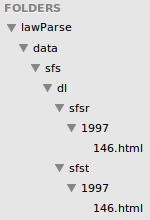
\includegraphics[scale=1]{../imgs/structure.png}
\captionof{figure}{Tree structure for downloaded files}
\end{center}
Under the root 'lawParse' there is a directory called 'data' which contains all different types of legal documents, here we have a 'sfs' directory where we store the downloaded, ('dl') parsed and eventually the generated files respectively. In all these directories we have another level for 'sfsr' and 'sfst' files, here the statutes are sorted according to the year they were created.        

\subsection{Parsing}

The first step is to scan the directory containing the files, this will give us a list of files, we will loop through the list one statute at the time. For our exampel (1997:146) statute we we will have the following set of files:\\ 
\begin{minted}[bgcolor=bg]{console}
All files connected to this file: 
	{'sfst': [u'../lawParse/data/sfs/dl/sfst/1997/146.html'], 
	 'sfsr': [u'../lawParse/data/sfs/dl/sfsr/1997/146.html']}
\end{minted}
\linebreak
We then transform and trim the file names so that they will be on the format '1997/146' instead of '../1997/146.html'. The actual parsing step then begins if the file met these three requirements:
\begin{enumerate}
\item If we have the file parsed already and it is newer than the incoming raw file, don't parse it again.
\item Filter out documents that are not proper SFS documents. They will have a name like ‘N1992:31’\footnote{TODO: Explain why.}
\item Skip parsing the documents that have been or will be revoked, they are marked as \textit{“The constitution is repealed / shall be repealed”}\footnote{“Författningen är upphävd/skall upphävas”}
\end{enumerate}
The parsing begins with creating a SFS specific Parser, that has a set of properties and rules defined such as regular experssions created for parsing SFS statutes. Like this regular expression for matching a SFS number:\\
\begin{minted}[bgcolor=bg, firstline=2]{python}
$
reSimpleSfsId = re.compile(r'(\d{4}:\d+)\s*$')
\end{minted}
\linebreak
The raw string ('r') notation keeps the regular expression clean, without it every backslash would have to be prefixed with another on to escape it. Then we are looking for four (4) digits followed by a colon(:) and one (1) or more digits. The 's' at the end is there to match white spaces (behaves differently with or without the unicode flag turned on). Finally the dollar sign (\$) states that the match have to be the end of the string. The other regular expressions are created in a similar fashion, in total there are about 30 expression matching everything from chapter ids and numbered lists to the definition of a revoked date.\\\\  
When the SFSParser class is initialized and have all it’s properties created, we can divide the parsing into two steps. One where we handle the register file (SFSR) and one for the full text (SFST). We begin with creating a registry with \textit{registerposts} containing meta information and other information regarding changes to the statute.\\ 
\begin{minted}[bgcolor=bg]{python}
Registerpost: 
{u'Ansvarig myndighet': Link('u'F\xf6rsvarsdepartementet'',
	uri=u'http://lagen.nu/org/2008/forsvarsdepartementet'), 
 u'Ikraft': DateSubject(1997, 7, 1), 
 u'SFS-nummer': u'1997:146'}

Registerpost: 
{u'Omfattning': [
	u'\xe4ndr. ', 
	Link('u'1 \xa7'',
	uri=u'http://rinfo.lagrummet.se/publ/sfs/1997:146#P1')],
 u'Ikraft': DateSubject(2012, 7, 16), 
 u'Rubrik': u'F\xf6rordning (2012:334) om \xe4ndring i 
	hemv\xe4rnsf\xf6rordningen (1997:146)', 
 u'SFS-nummer': u'2012:334'}
\end{minted}
\linebreak
\newline
The first registerpost created for 1997:146 describes basic properties such as responsible authority, entry into force and SFS number. The second\footnote{There's actually three register posts for 1997:146, I left a 'change post' out to save space} registerpost states that there has been some changes to the statute. We can find out if it is a change or if some part has been revoked\footnote{Omfattning can be for example "Change" or "Revoked" ("Ändr." or "Upph.")}, also we can see the force into entry and the change statute's SFS number. All these values are represented with different data types discussed in the 'Implementation' section, for ex. 'Link', 'DateSubject' or a unicode 'u' string.\\\\
The second part is to deal with the full text part of the statute, we do this by creating an intermediate text file with just the raw\footnote{It is not the complete downloaded file, we get rid of the "HTML" mark up of the document so that we only have text.} text. This file is saved in a directory called 'intermediate' on the same level as the downloaded, 'dl' directory in the file tree structure. \\\\ 
The file we have downloaded consist of a header\footnote{See bilaga X for example input file.} with information similar to the register file. We could probably reuse some information\footnote{SFS number and responsible authority could be reused for example.} but we have everything set up for parsing and it is a fairly simple procedure so we go ahead and save it again. This information will be part of the header in the HTML file when that is created later on. For the information in the header we create a corresponding object, in the example below we create \textit{UnicodeSubjects}\footnote{We will look closer at this in the next section 'RDF markup'}, with the values \textit{SFS number} and \textit{Headline}, their predicates will be an URI to that object's definition.\\
\begin{minted}[bgcolor=bg]{python}
if key == u'Rubrik':
	meta[key] = UnicodeSubject(val, predicate=self.labels[key])
elif key == u'SFS nr':
	meta[key] = UnicodeSubject(val, predicate=self.labels[key])
\end{minted} 
\linebreak
\newline
Here is the values for the variables above when the header infromation is created:\\
\begin{minted}[bgcolor=bg]{console}
key:SFS nr
val:1997:146
self.labels[key]:
	http://rinfo.lagrummet.se/taxo/2007/09/rinfo/pub#fsNummer
key:Rubrik
val:Hemvransforordning (1997:146)
self.labels[key]:
	http://purl.org/dc/terms/title
\end{minted}
\linebreak
\newline
To mark up the full text we call a number of methods on the raw text file, to first of, find out what the part we are looking at should be represented as and then to create an object with that type's properties. The main method is \textbf{makeForfattning} when it is called it will in turn call several other methods like \textbf{makeKapitel,} \textbf{makeParagraf} and \textbf{makeTabell} and so on. The logic to figure out what each part should be marked up as uses a 'statehandler' to keep track of what part we just parsed and to guess what should come next. If we are inside the \textbf{makeStycke} method possible states/methods we can invoke are different types of lists and tables. Then when we reach the end of the current state we start over again and look what state the next part should be, this part can probably not be a list or a table, those states can only be reached from within certain states. Following that logic for example a paragraph can not be called within a chapter, each type has its place in the hierarchy. \\\\
All objects have an \textbf{"isObject"} and \textbf{"makeObject"} method, and they are for example used like the example below shows.\\ 
\begin{minted}[bgcolor=bg]{python}
def guesState(self):
	try:
		if self.reader.peekLine() == '':
			handler = self.blankLine
		elif self.isAvdelning():
			handler = self.makeAvdelning
		elif self.isKapitel():
			handler = self.makeKapitel
		elif self.isParagraf():
			handler = self.makeParagrafnd{minted}
		...
\end{minted}
\linebreak  
\newline
When we are done with the parsing the text body we add some additional information to the law’s meta information such as time created and preliminary work. To find out if there is any preliminary work we check the \textit{registerposts} in the register we have created, and save the URI to that document if existing.

\subsection{RDF markup }
During all the different parsing steps, I have mentioned that we create data objects with specialized properties for the different parts of the statute. Let's take a closer look at one of the objects that are created during our parse example.\\
In the previous section we look at example code for finding a statute's SFS number and headline, they are both of the type \textit{UnicodeSubject}. The class \textit{UnicodeSubject} it self does not do anything as we can see in the class definition below.\\
\begin{minted}[bgcolor=bg]{python}
class UnicodeSubject(PredicateType, UnicodeStructure):
	pass
\end{minted} 
\linebreak
\newline
However the class inherits from two other classes, \textit{PredicateType} and \textit{UnicodeStructure}. We are going to look at what our \textit{PredicateType} objects looks like. In the second chapter we stated that RDF is based upon the idea of making statements about resources in the form of triples of subject-predicate-object. Here we are obviously looking at the 'Predicate' part, as the class definition below reads; Inheriting from this class gives the child class a predicate attribute that describes the RDF predicate to which the class is the RDF subject.\\    
\begin{minted}[bgcolor=bg]{python}
class PredicateType(object):
    """Inheriting from this class gives the child class a 
    predicate attribute that describes the RDF predicate to 
    which the class is the RDF subject"""
    def __init__(self, *args, **kwargs):
	if 'predicate' in kwargs:
	    self.predicate = kwargs['predicate']
	    shorten = False
	    for (prefix, ns) in Util.ns.items():
		if kwargs['predicate'].startswith(ns):
		    predicateUri = kwargs['predicate']
		    kwargs['predicate'] = kwargs['predicate']
			.replace(ns, prefix + ':')	
		    shorten = True
		else:
		    from rdflib import RDFS
		    self.predicate = RDFS.Resource
	    super(PredicateType, self).__init__(*args, **kwargs)
\end{minted} 
\linebreak
\newline
When the object is initialized we compare the predicate's URI to some common name spaces that we have stored, if that is the case we can swap the long URI for a much shorter prefix. In our case with the SFS number and the headline we can substitute the title's URI \url{http://purl.org/dc/terms/title} for simply 'dct:title' and \url{http://rinfo.lagrummet.se/taxo/2007/09/rinfo/pub#fsNummer} becomes 'rinfo:fsNummer'. Below we find part of the name space list, as we can see we can reuse definitions that are already defined by large international organisations, it is only 'rinfo' that is specific "Swedish-legal" definition.     
\begin{minted}[bgcolor=bg]{python}
# Common namespaces and prefixes for them
ns = {
    'dc':'http://purl.org/dc/elements/1.1/',
    'dct':'http://purl.org/dc/terms/',
    'rdfs':'http://www.w3.org/2000/01/rdf-schema#',
    'rdf':'http://www.w3.org/1999/02/22-rdf-syntax-ns#',
    'skos':'http://www.w3.org/2008/05/skos#',
    'rinfo':'http://rinfo.lagrummet.se/taxo/2007/09/rinfo/pub#',
    'xht2':'http://www.w3.org/2002/06/xhtml2/'
}
\end{minted} 
\linebreak
\newline
This way we can mark up our legal documents with short prefixes that makes the documents readable for both humans and computers in a way that contributes to the Semantic Web. In a final HTML file our title would look something like the snippet below, much more meaningful then just a header tag with a title, yet still simple enough to be understandable for human readers.\\
\begin{minted}[bgcolor=bg]{html}
<h1 property="dct:title">Hemvarnsforordning (1997:146)</h1>
\end{minted}
\linebreak
\newline
\subsection{Generating XHTML}
To create an XHTML representation of the parsed statute we use a third party library called \textit{Genshi}\footnote{See the 'Implementation' section for more information regarding third party libs.}. We use Genshi’s ‘TemplateLoader’ to load a template we have created that specifies how we want the our XHTML to look like, ex. which values goes where etc. A nice feature with Genshi is that it uses a Stream-based filtering\footnote{\url{http://genshi.edgewall.org/wiki/Documentation/filters.html}} that allows us to apply various transformations as a template is being processed, without having to parse and serialize the output again.\\\\
Below is an example of how the template file renders a headline. As the code
snippet shows there is two <h> tag templates to chose from, one if it is a "normal" headline and one if it is an sub headline, then an extra class is added to the tag.\\
\begin{minted}[bgcolor=bg]{html}
<div py:def="render_rubrik(rubrik)" py:strip="" py:choose="">
    <h py:when="rubrik.type == 'underrubrik'" py:content="rubrik"
	id="${rubrik.id}" class="underrubrik">Underrubrik</h>
    <h py:otherwise="" py:content="rubrik"
	id="${rubrik.id}">Huvudrubrik</h>
</div>
\end{minted}
\linebreak  
\newline
TODO: Describe more what it does.\\
\subsection{Bonus - Generating HTML}
Not part of the thesis, but an example implementation using XSL transformation, a look at the final output. 


\section{Output}
Example of the parsed xht file and maybe also an example html file.
\subsection{RDF}
RDF examples from the law

\subsection{Rättsinformationsprojektet standard}
Examples of places where the law is marked up with rip's standard. 
Text from their specifications.

\section{Performance}
Timing for 1, 100, 1000, all laws? Maybe a nice chart. 
What step is the most time/power consuming?
